%!TEX root = ../Work-stealing Queues.tex
\section{Performance Analysis}
\label{sec:performance_analysis}
\todo{Write why ABP being so good is not surprising. Write about how complicated the different queues are.}
\subsection{Chase-Lev vs ABP}
When comparing the performance of the Chase-Lev and ABP implementations in Figure \ref{fig:32nonidem} we see that Chase-Lev is faster at quick sort and XML serialization. On the surface it might seem odd that Chase-Lev should outperform ABP as Chase-Lev also has to maintain the circular array. However, as Chase-Lev does not have to deal with the ABA problem this better performance could be due to a lot of failed CAS operations in ABP\@. In general Chase-Lev cannot be expected to perform better then ABP\@. We can also see that Chase-Lev tends to be slower than ABP on cases with low cost tasks (Spanning-Tree and Raw) and speeds up as tasks become more work intensive. If more time is needed by each task the relative time spend on queue operation lowers and thus the increased overhead of Chase-Lev has less of an effect on the overall performance.

\begin{figure}
\begin{tikzpicture}
\begin{axis}[title=Results for 32 threads,  
  ylabel={Relative speedup},
  symbolic x coords={ABP, Chase-Lev, Chase-Lev (Shrinking)},
  xtick=data,
  x tick label style={rotate=315,anchor=west},
  legend style={at={(1.17,1)}, anchor=north,legend columns=1},
  legend cell align=left,
  ybar, bar width=8,
  height=150,
  width=300]
\addplot coordinates { % Quick sort
(ABP,1) (Chase-Lev, 1.044061) (Chase-Lev (Shrinking), 1.173693)
};
\addplot coordinates { % Spanning tree
(ABP,1) (Chase-Lev, 1.013258) (Chase-Lev (Shrinking), 1.056889)
};
\addplot coordinates { % XML
(ABP,1) (Chase-Lev, 1.188274) (Chase-Lev (Shrinking), 1.165794)
};
\addplot coordinates { % Raw
(ABP,1) (Chase-Lev, 0.753401) (Chase-Lev (Shrinking), 0.869602)
};
\legend{Quick sort, Spanning tree, XML, Raw}
\end{axis}
\end{tikzpicture}
\caption{Results for 32 threads with non-idempotent queues.}
\label{fig:32nonidem}
\end{figure}

Another advantage of Chase-Lev is that it does not need to know size of the queue before hand. This allows for more memory efficiency and makes it easier for the user. This means that Chase-Lev in general is a good choice for cases where the number of subtasks created by each task is hard to predict precisely, and especially for cases with more intensive individual tasks.

We have also made a shrinking version of Chase-Lev which has yielded some interesting results. Since this queue requires more overhead to not only expand the queue, but to also shrink it, we expected it to perform worse than both ABP and the standard Chase-Lev queue. However, it has performed just as well as the two others and even outperformed them in certain cases. The reason for this could be garbage collection. Since ABP has to have a queue at the size of the worst case scenario, most of the time only very little of that will actually be used. In contrast the Chase-Lev shrinking queue is only as big as needed, and the left overs are garbage collected on the run. This means that there is a lot more items for the garbage collector to check in the ABP queue which affect the performance compared to the Chase-Lev queues.

\subsection{Quick Sort scaling}
The performance of our quick sort case does not scale well (Figure \ref{fig:qsscaling}). The performance increase from eight to sixteen workers is negligible, and past sixteen the time taken actually increases. There are a few factors that could be the source of this. Firstly, as the first worker has to split the entire list in two, and then only spawns work for one new worker, there is a large period of time where most of the workers have nothing to do. This is not a problem if each worker have their own core, but when there are more workers than cores (here past sixteen workers) it could affect performance. Maintaining the remaining workers sitting in a steal loop waiting for work to be available, could cause more overhead than the performance gained from more threads when there is work to do. Another reason could be that quick sort relies on a large amount of memory accesses. If this is the bottleneck rather than the operations on the CPU it could explain why it does not scale well. This however does not explain the extra time it takes with more than sixteen cores.\todo{Fact check?}

\begin{figure}
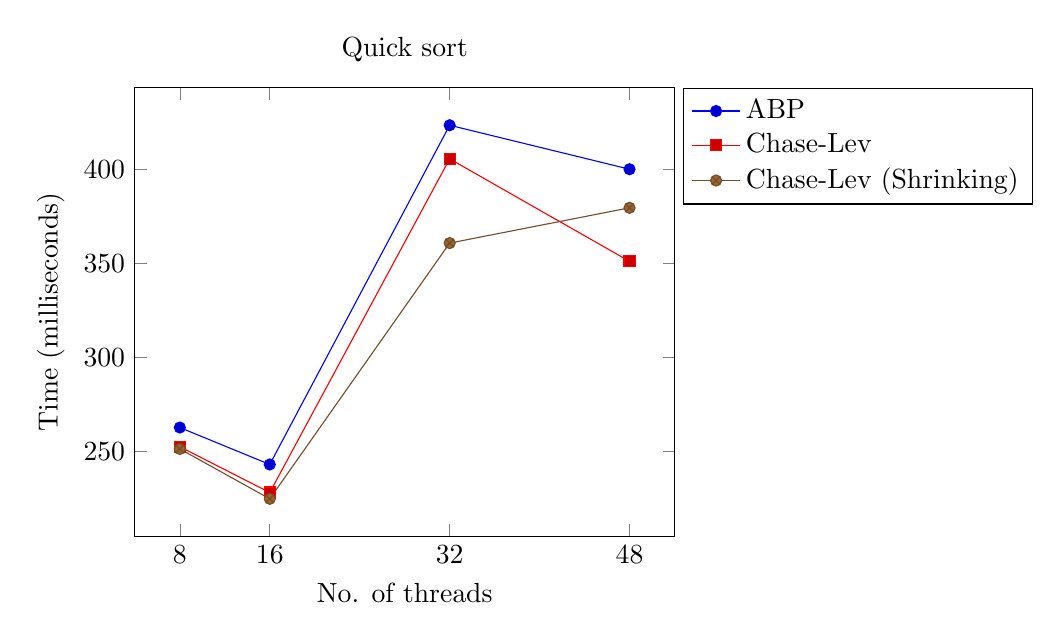
\begin{tikzpicture}
\begin{axis}[
  title={Quick sort},
  xlabel={No. of threads},
  ylabel={Time (milliseconds)},
  xtick={8,16,32,48},
  legend style={at={(1.34,1)}, anchor=north,legend columns=1},
  legend cell align=left
  ]
\addplot+[sharp plot] coordinates % ABP
{(8,262.86) (16,243.2) (32,423.68) (48, 400.28)};
\addplot+[sharp plot] coordinates % Chase-Lev
{(8,252.67) (16,228.27) (32,405.8) (48, 351.26)};
\addplot+[sharp plot] coordinates % Chase-Lev (Shrinking
{(8,251.47) (16,224.93) (32,360.98) (48, 379.75)};
\legend{ABP, Chase-Lev, Chase-Lev (Shrinking)}
\end{axis}
\end{tikzpicture}
\caption{Quick sort scaling.}
\label{fig:qsscaling}
\end{figure}

\subsection{Performance of Idempotent Queues}
Looking at Figure \ref{fig:idemraw}, the idempotent queues are very slow in the raw case. At first this does not seem right as one of the advantages of the idempotent queues should be faster queue operations which is exactly what raw tests. The reason for this bad performance is that there is no synchronization of information on what work is done and what needs to be done. If two threads grab the same task, they both spawn the children of that task, which will be added to their queues. This means that if two workers do the same task it is not only the task itself that has to be executed twice, but also all the children of that task.

\begin{figure}
\begin{tikzpicture}
\begin{axis}[title=Results for 32 threads,  
  ylabel={Relative speedup},
  symbolic x coords={ABP, Idempotent (LIFO), Idempotent (FIFO),
                     Idempotent (Double-ended), Duplicating},
  xtick=data,
  x tick label style={rotate=315,anchor=west},
  legend style={at={(1.17,1)}, anchor=north,legend columns=1},
  legend cell align=left,
  ybar, bar width=10,
  height=150,
  width=300]
\addplot coordinates { % Raw
(ABP,1) (Idempotent (LIFO), 0.210492)
(Idempotent (FIFO), 0.171293) (Idempotent (Double-ended), 0.118589) (Duplicating, 0.708532)
};
\legend{Raw}
\end{axis}
\end{tikzpicture}
\caption{Idempotent performance on raw compared to ABP.}
\label{fig:idemraw}
\end{figure}

This is backed by the fact that the duplicating queue is a lot faster at raw than the other idempotent queues. This is because the duplicating queue only duplicates work when exactly one thief steals a task at the same time as the owner. In the cases of the other idempotent queues it can happen to any number of thieves at the same time, and is therefore a lot more frequently occurring. With less work duplication the duplicating queue performs a lot better in the raw case.